\documentclass[UTF8]{ctexart}
\ctexset { section = { format={\Large \bfseries } } }
\pagestyle{plain}
\usepackage{float}
\usepackage{amsmath}
\usepackage{amssymb}
\usepackage{listings}
\usepackage{graphicx}%插入图片宏包
\usepackage{xcolor}
\usepackage{geometry}
\geometry{a4paper,scale=0.8}
\usepackage{caption}
\usepackage{subcaption}
\usepackage[colorlinks=true, linkcolor=blue, citecolor=blue, urlcolor=blue]{hyperref}
\captionsetup[figure]{name={Figure}}
\captionsetup[table]{name={Table}}
\definecolor{Rhodamine}{RGB}{227,11,92}


\lstset{
language=Python, % 设置语言
basicstyle=\ttfamily\small, % 设置字体族
breaklines=true, % 自动换行
keywordstyle=\bfseries\color{blue}, % 设置关键字为粗体,
morekeywords={}, % 设置更多的关键字,用逗号分隔
emph={self}, % 指定强调词,如果有多个,用逗号隔开
emphstyle=\bfseries\color{Rhodamine}, % 强调词样式设置
commentstyle=\color{black!50!white}, % 设置注释样式,斜体,浅灰色
stringstyle=\bfseries\color{red!90!black}, % 设置字符串样式
columns=flexible,
numbers=left, % 显示行号在左边
numbersep=2em, % 设置行号的具体位置
numberstyle=\footnotesize, % 缩小行号
frame=single, % 边框
framesep=1em % 设置代码与边框的距离
}

\title{\textbf{Image Processing Homework 4}}
\author{吴嘉骜 21307130203}
\date{\today}

\begin{document}

\maketitle

\noindent
\section{}
\setlength{\parindent}{0pt}
Implement a program to realize frequency domain filtering based on the five steps outlined in the lecture slides:\\
(1) Conduct a lowpass smoothing operation, and apply the algorithm to an image.
Display the spectrum of the original image, the spectrum of the result after frequency domain operation, and the result of the operation.\\
(2) Implement at least one image sharpening operation based on frequency domain manipulation.\\
Note: The spatial-to-frequency domain transformation (i.e., discrete frequency domain/Fourier transform and its inverse) can be implemented using library functions.\\
\textbf{Solution}:\\
The code from \texttt{freqfilter.py} is long and thus shown in the \hyperlink{code1}{Appendix}. Here we interpret the code structure and functions briefly.\\
The \texttt{Frequencyfilter} class is designed for performing frequency domain filtering on images. Both image smoothing and sharpening are implemented using this class. 
Below list the main methods of this class:

\begin{itemize}
    \item \textbf{\_init\_}: The constructor method takes an image path as input, reads the image in grayscale as a \texttt{numpy} array, and initializes the image dimensions.
    
    \item \textbf{show\_image}: This method displays the image. It can perform a logarithmic transformation to improve the visibility of frequency components, clip the image's pixel values, or scale the image to the 0-255 range. It can also save the modified image to a specified path.
    
    \item \textbf{show\_spectrum}: This method computes and displays the Fourier spectrum of the image. It uses the \texttt{show\_image} method with a logarithmic modification to make the spectrum more visible.
    
    \item \textbf{padding}: To prevent wrap-around error during the filtering process, this method pads the image with zeros, doubling its size in both dimensions.
    
    \item \textbf{freqfilter}: This is the core method for applying a frequency domain filter. It involves padding the image, performing a Fourier transform, applying a given filter transfer function, and then reconstructing the image via inverse Fourier transform.
    
    \item \textbf{ilpf}: Generates an ideal low-pass filter transfer function with a specified cutoff frequency to allow only frequencies below the cutoff to pass through.
    
    \item \textbf{glpf}: Generates a Gaussian low-pass filter transfer function, with the standard deviation of the Gaussian function equivalent to the cutoff frequency. This creates a smoother transition than the ideal filter.
    
    \item \textbf{ihpf}: Implements an ideal high-pass filter by using the ideal low-pass filter method \texttt{ilpf}, subtracting its result from 1.
    
    \item \textbf{ghpf}: Implements a Gaussian high-pass filter by subtracting the Gaussian low-pass filter result from 1, providing a smoother transition in the frequency cutoff than the IHPF.
    
    \item \textbf{laplacian\_filter}: Computes the transfer function of a Laplacian filter, based on the negative Laplacian operator.
    
    \item \textbf{laplacian\_sharpen}: Generates a sharpened image by applying the \texttt{laplacian\_filter} to the image in the frequency domain.
\end{itemize}
Then we show the results of the two operations.

\textbf{\large (1) Image smoothing operation}
\begin{figure}[htbp]
    \centering
    % 第一行三张图片
    \begin{subfigure}{0.3\textwidth}
        \centering
        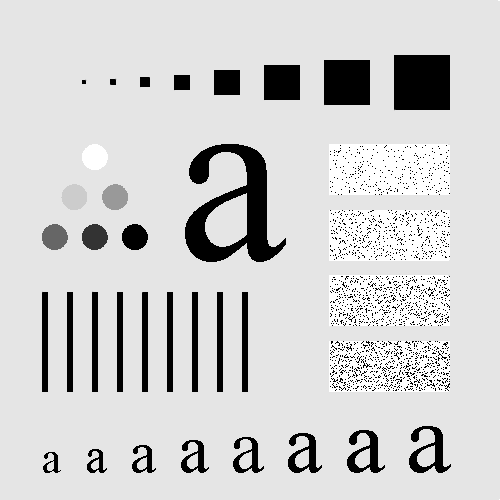
\includegraphics[width=\linewidth]{test_pattern_blurring.png}
        \caption{Input original image}
    \end{subfigure}%
    \hfill
    \begin{subfigure}{0.3\textwidth}
        \centering
        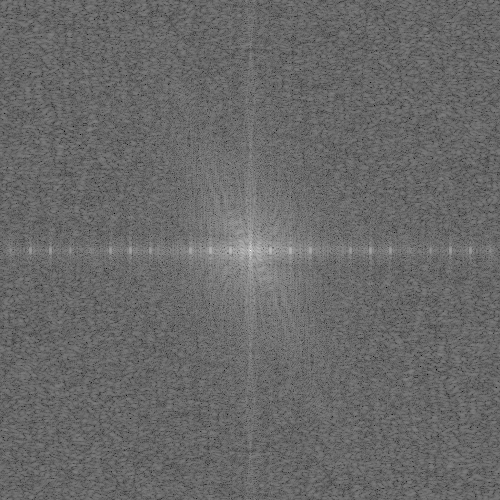
\includegraphics[width=\linewidth]{pattern_spectrum.png}
        \caption{Spectrum of the original image}
    \end{subfigure}%
    \hfill
    \begin{subfigure}{0.3\textwidth}
        \centering
        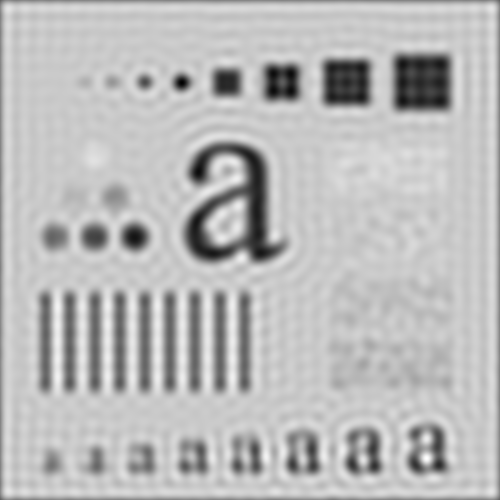
\includegraphics[width=\linewidth]{pattern_ilpf.png}
        \caption{Ideal low pass filter $D_0 = 60$}
    \end{subfigure}

    \vspace{0.5cm} % 调整两行之间的距离

    % 第二行三张图片
    \begin{subfigure}{0.3\textwidth}
        \centering
        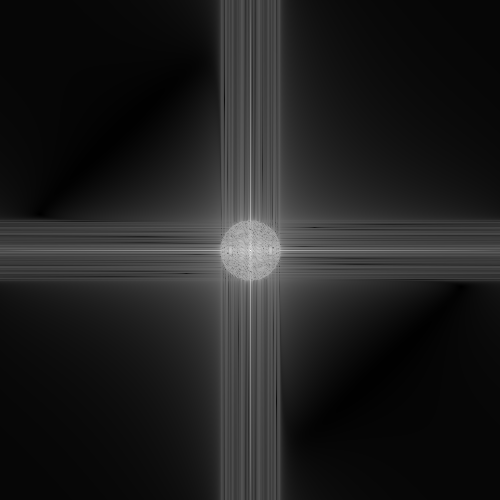
\includegraphics[width=\linewidth]{pattern_ilpf_spectrum.png}
        \caption{Spectrum after ILPF}
    \end{subfigure}
    \hfill
    \begin{subfigure}{0.3\textwidth}
        \centering
        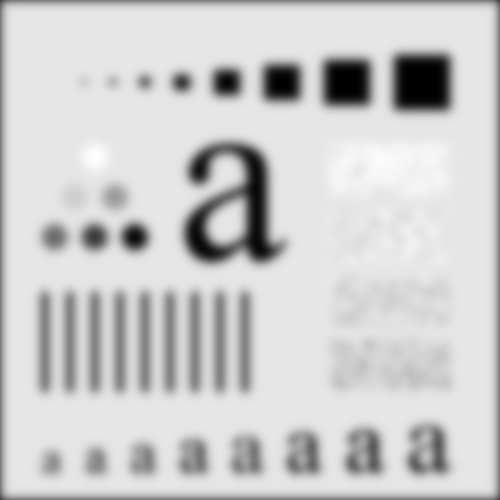
\includegraphics[width=\linewidth]{pattern_glpf.png}
        \caption{Gaussian low pass filter $D_0 = 30$}
    \end{subfigure}%
    \hfill
    \begin{subfigure}{0.3\textwidth}
        \centering
        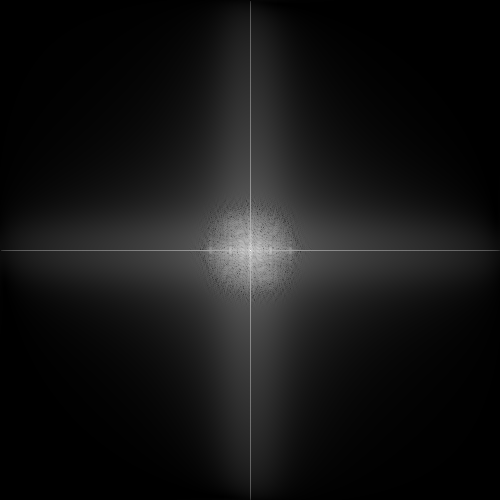
\includegraphics[width=\linewidth]{pattern_glpf_spectrum.png}
        \caption{Spectrum after GLPF}
    \end{subfigure}%

    \caption{Image after frequency smoothing operation}
\end{figure}

We can see that the Gaussian low pass filter provides a smoother transition in the frequency cutoff than the ideal low pass filter,
and the ILPF presents obvious ringing artifacts in the spatial domain.\\

\textbf{\large (2) Image sharpening operation}

\begin{figure}[htbp]
    \centering
    \begin{subfigure}{0.3\textwidth}
        \centering
        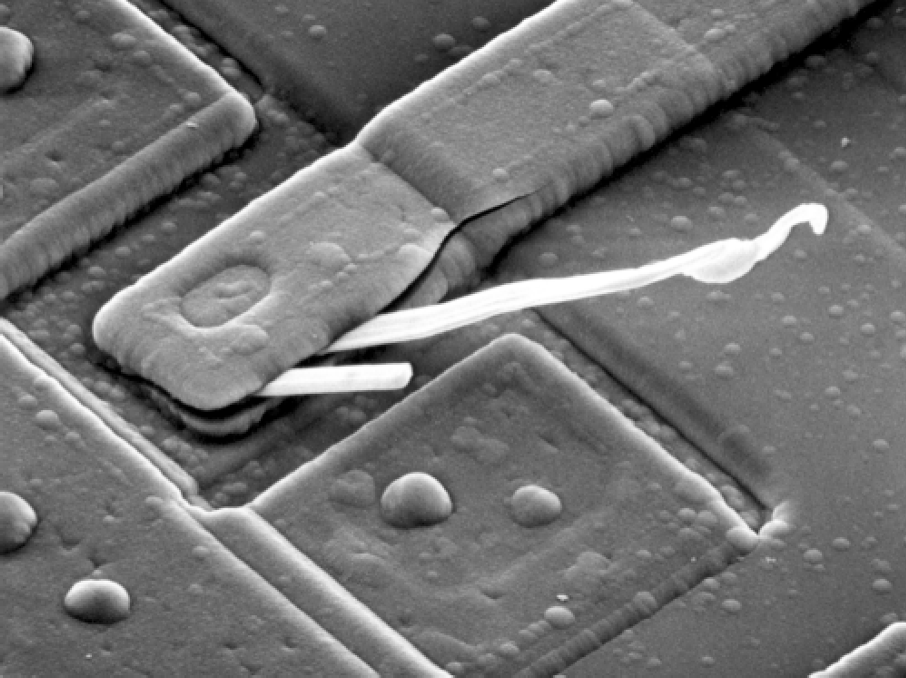
\includegraphics[width=\linewidth]{blown_ic.png}
        \caption{Input original image}
    \end{subfigure}%
    \hfill
    \begin{subfigure}{0.3\textwidth}
        \centering
        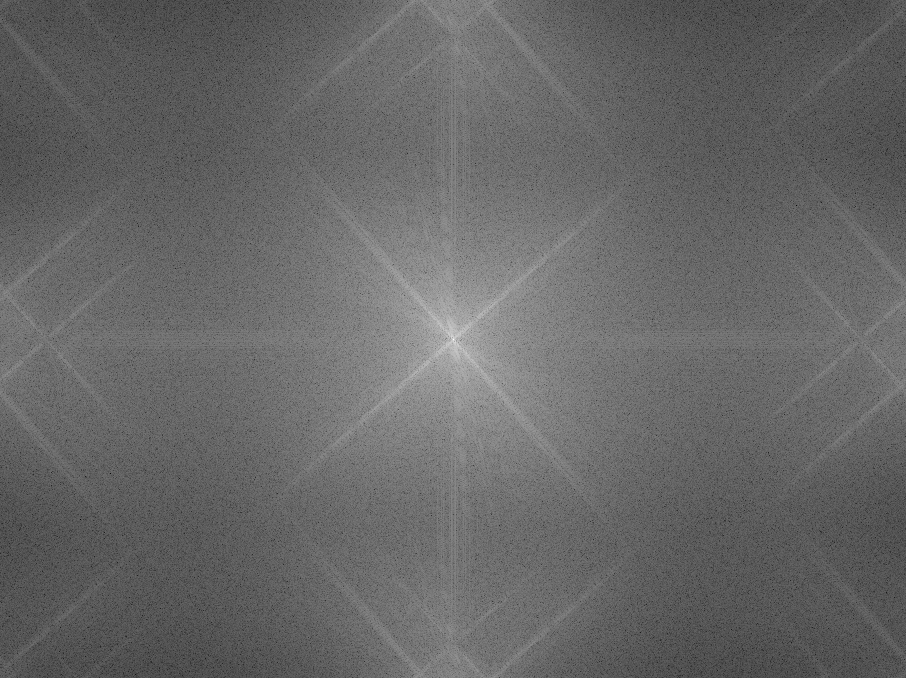
\includegraphics[width=\linewidth]{ic_spectrum.png}
        \caption{Spectrum of the original image}
    \end{subfigure}%
    \hfill
    \begin{subfigure}{0.3\textwidth}
        \centering
        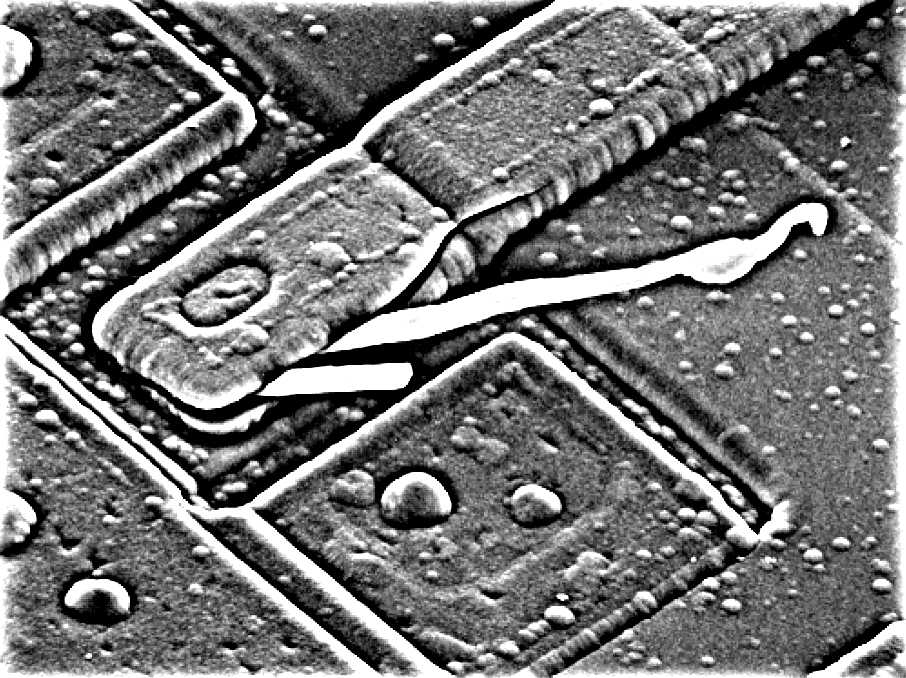
\includegraphics[width=\linewidth]{ic_ghpf.png}
        \caption{Gauss high pass filter $D_0 = 30$}
    \end{subfigure}

    \vspace{0.5cm}
    \centering
    \begin{subfigure}{0.3\textwidth}
        \centering
        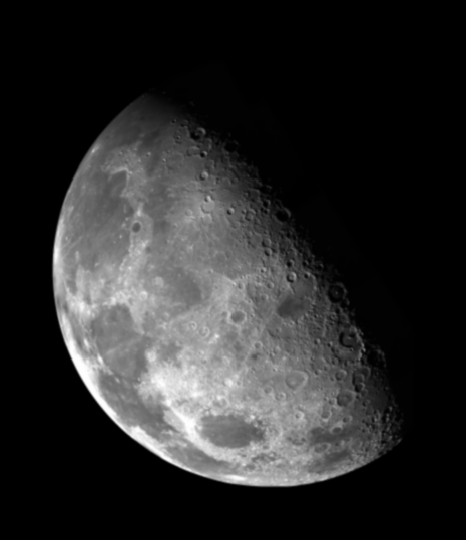
\includegraphics[width=\linewidth]{blurry_moon.png}
        \caption{Input original image}
    \end{subfigure}%
    \hfill
    \begin{subfigure}{0.3\textwidth}
        \centering
        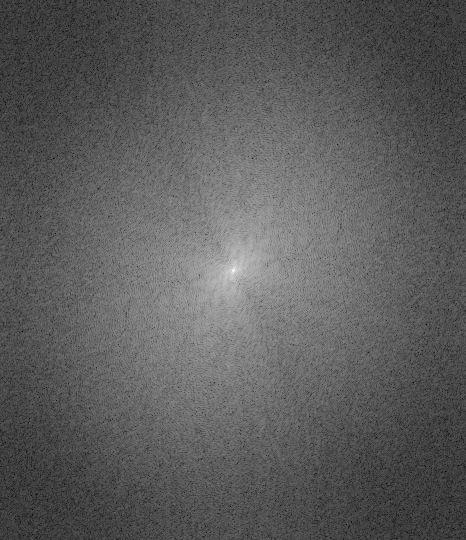
\includegraphics[width=\linewidth]{blurry_moon_spectrum.png}
        \caption{Spectrum of the original image}
    \end{subfigure}%
    \hfill
    \begin{subfigure}{0.3\textwidth}
        \centering
        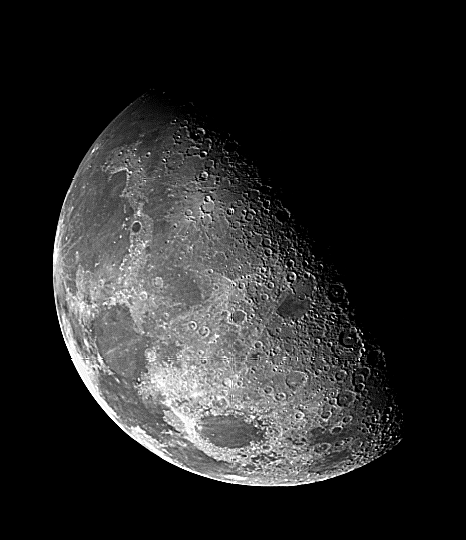
\includegraphics[width=\linewidth]{blurry_moon_lap.png}
        \caption{Laplacian sharpening}
    \end{subfigure}
    \caption{Image after frequency sharpening operation}
\end{figure}

From the figures above, we can see that both the Gaussian high pass filter and Laplacian filter can effectively sharpen the image, 
with the edges more clearly defined.\\

\section{}
Implement a program to realize a selective filtering method in the frequency domain,
aiming to remove strip artifacts from a brain CT phantom image (Shepp-Logan);
alternatively, create an image with periodic noise and use a frequency domain selective filter to remove the noise.\\
Note: The spatial-to-frequency domain transformation (i.e., discrete frequency domain/Fourier transform and its inverse) can be implemented using library functions.\\
\textbf{Solution}:\\
The full code from \texttt{brain\_CT.py} is shown in the \hyperlink{code2}{Appendix}. Here we interpret the code structure briefly, and later we will explain the key functions in detail.\\
\begin{itemize}
\item \textbf{read\_img}: Reads an image from the given path and converts it to a grayscale numpy array.
\item \textbf{show\_image}: Displays the image using matplotlib with specified figure size and colormap.
\item \textbf{img\_modify}: Normalizes and processes the image for display based on the specified modification type, including logarithmic transformation, clipping, and scaling.
\item \textbf{show\_spectrum}: Computes and displays the frequency spectrum of the image.
\item \textbf{show\_spectrum2}: Displays the frequency spectrum from a given discrete Fourier transform (DFT).
\item \textbf{ghpf\_shift}: Generates a Gaussian high pass filter (GHPF) centered at the given coordinates.
\item \textbf{notch\_reject}: Creates a notch reject filter with the specified coordinates and cutoff frequency to attenuate unwanted frequencies.
\item \textbf{main}: Reads the image, generates the filter transfer function, applies the filter to the DFT of the image, and displays the result.
\end{itemize}
Some important functions are shown below.
\begin{lstlisting}
from PIL import Image
import numpy as np
import matplotlib.pyplot as plt
    
def ghpf_shift(img, d0, u0, v0):
    '''
    Gaussian high pass filter (GHPF) with center shifted to (u0, v0).
    
    Parameters:
        - img: the input image, a 2D numpy array
        - d0: the cutoff frequency
        - u0, v0: the center coordinates of the highpass filter
        
    Returns:
        - filter_transfun: the filter transfer function of GHPF, with size m*n
    '''
    m, n = img.shape
    filter_transfun = np.zeros((m, n))
    for u in range(m):
        for v in range(n):
            d2 = (u-u0)**2 + (v-v0)**2
            filter_transfun[u, v] = 1 - np.exp(-d2/(2*d0**2))
    return filter_transfun

def notch_reject(img, coord, d0):
    '''
    Notch reject filter.
    
    Parameters:
        - img: the input image, a 2D numpy array
        - coord: the center coordinates of each highpass filter, k*2 array, k is the number of filters
        - d0: the cutoff frequency of the highpass filter
        
    Returns:
        - filter_transfun: the filter transfer function of notch reject filter, with size m*n
    '''
    m, n = img.shape
    k = coord.shape[0]
    nr = np.ones((m,n))
    for i in range(k):
        u, v = coord[i]
        nr *= ghpf_shift(img, d0, u, v) * ghpf_shift(img, d0, m-u, v) * ghpf_shift(img, d0, u, n-v) * ghpf_shift(img, d0, m-u, n-v)
    return nr

img_path='./hw4.png'
img = read_img(img_path)
show_spectrum(img)

# create the filter transfer function
xs = [16, 100, 180, 216, 300]
coor = np.array([[x, y] for x in xs for y in xs])
nr = notch_reject(img, coor, 21)

# apply the filter transfer function to the DFT of the image
# ...
g = f * nr
# ...
\end{lstlisting}

Together with the following figures, we explain the method to remove the strip artifacts from the image.\\

\begin{figure}[htbp]
    \centering
    \begin{subfigure}{0.5\textwidth}
        \centering
        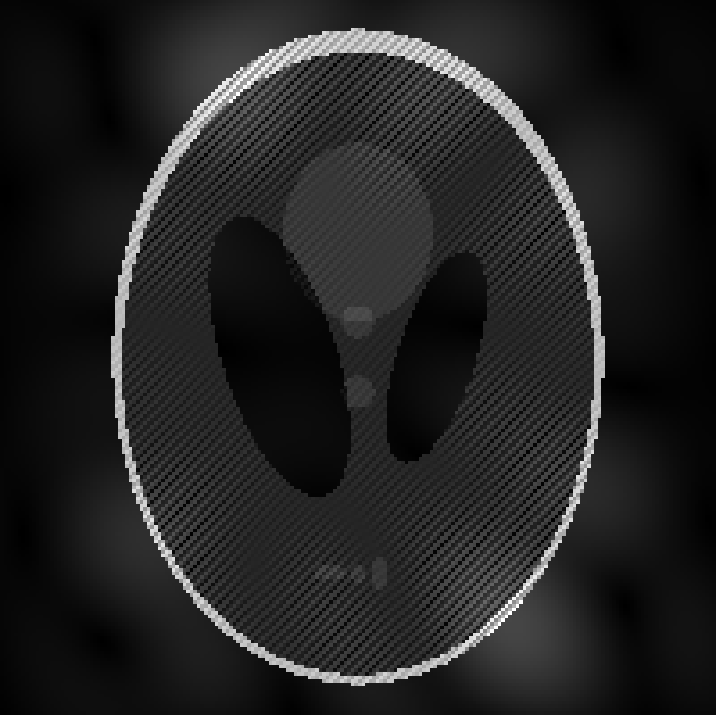
\includegraphics[width=0.8\linewidth]{hw4.png}
        \caption{Input original image}
    \end{subfigure}%
    \hfill
    \begin{subfigure}{0.5\textwidth}
        \centering
        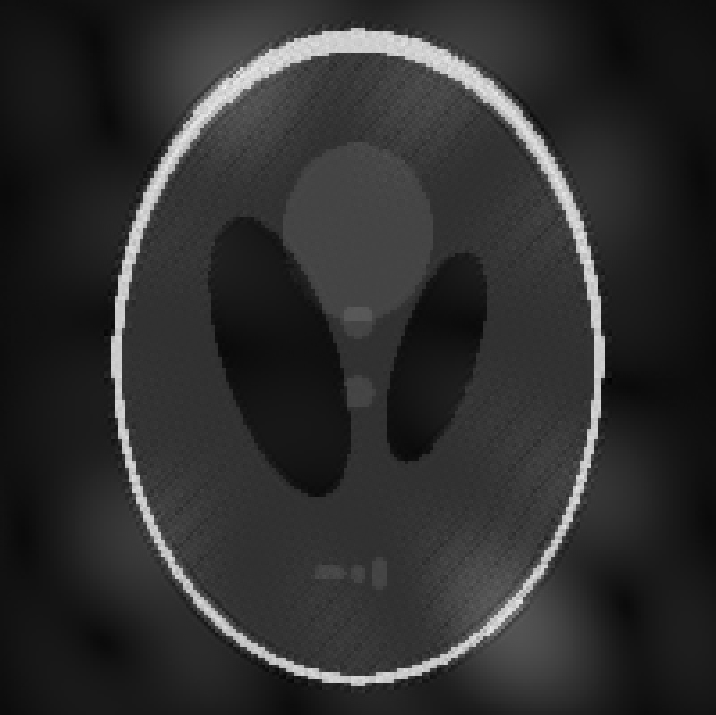
\includegraphics[width=0.8\linewidth]{brainct.png}
        \caption{Image after frequency filtering}
    \end{subfigure}%

    \vspace{0.3cm}

    \begin{subfigure}{0.5\textwidth}
        \centering
        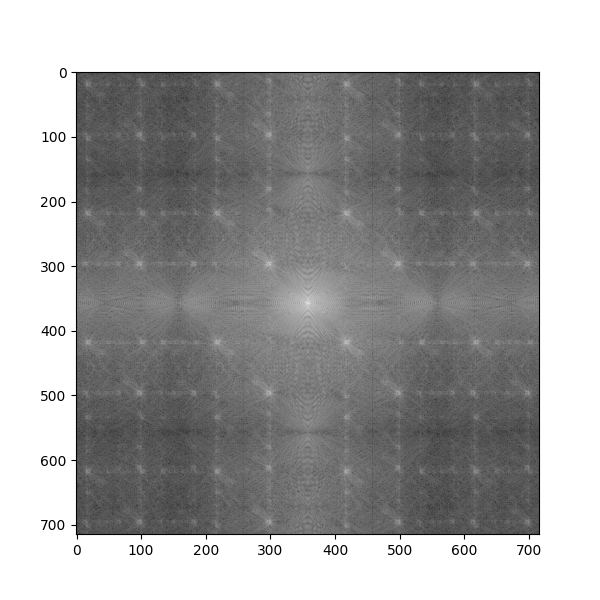
\includegraphics[width=1\linewidth]{hw4_spectrum.png}
        \caption{Spectrum of the original image}
    \end{subfigure}%
    \hfill
    \begin{subfigure}{0.5\textwidth}
        \centering
        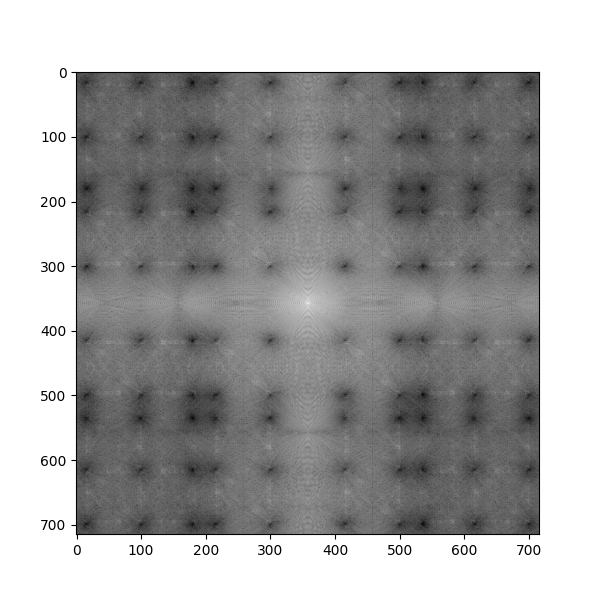
\includegraphics[width=1\linewidth]{ctfreq.png}
        \caption{Processed spectrum}
    \end{subfigure}

    \caption{Removing strip artifacts from a brain CT phantom image}
\end{figure}

From the spectrum of the original image, we can see that the strip artifacts are probably caused by the periodic noise in the frequency domain.
The energy bursts are symmetrically scattered in the four corners of the figure. Therefore, we can create a notch reject filter by muliplying four GHPFs centered at the four corners.
Once we ascertain the coordinates of one corner, we can generate the filter transfer function and apply it to the DFT of the image.\\
By visual inspection and mouse hovering on the spectrum, we find that the coordinates of the left-upper corner are permuated and combined by $[16, 100, 180, 216, 300]$, which is a rough estimation.
But we can then adjust the standard deviation of the GHPF to encompass the energy bursts completely. After several trials, we find that $D_0 = 21$ is a good choice.\\
We can see from the processed spectrum that the white bursts are removed, with the processed image clearer, although some artifacts still remain observable, and the image is slightly blurred.

\newpage
\appendix
\hypertarget{code1}{\section{Code for Problem 1}}
\begin{lstlisting}
from PIL import Image
import numpy as np

class Frequencyfilter():
    '''
    A class of functions for filtering in the frequency domain.
    '''
    
    def __init__(self, img_path):
        self.img_path = img_path
        self.img = np.array(Image.open(img_path).convert('L'))  # read as grayscale  
        self.shape = self.img.shape  # the original size of the image, a tuple (m, n), m rows and n columns
        self.nrow, self.ncol = self.shape
    
    def show_image(self, img=None, save_path=None, modified=0):
        '''
        Show the image.
        
        Parameters:
            - img: the input image, a 2D numpy array, by default None
            - save_path: the path to save the image, a string
            - modified: whether the image will be log-transformed (1), truncated (2) or scaled (3); 0 by default.
        '''
        if img is None:
            img = self.img

        if modified==1:
            img = np.log(1+img)
            if np.max(img) != 0:
                img = 255 *(img-np.min(img))/(np.max(img)-np.min(img))
        elif modified==2:
            img = np.clip(img, 0, 255)
        elif modified==3:
            scaled = (img-np.min(img))/(np.max(img)-np.min(img))
            img = 255 *scaled
        
        new_img = Image.fromarray(img.astype(np.uint8))
        if save_path:
            new_img.save(save_path)
        else:
            new_img.show()
    
    def show_spectrum(self, save_path=None):
        '''
        Show the frequency spectrum of the image.
        
        Parameters:
            - save_path: the path to save the spectrum, a string
        '''
        img = self.img
        f = np.fft.fft2(img)
        f = np.fft.fftshift(f)
        spectrum = np.abs(f)
        self.show_image(img=spectrum, save_path=save_path, modified=1)
    
    def padding(self, img=None):
        '''
        Pad the 2-D image with zeros to avoid the wrap-around effect. The size of the padded array is 2m*2n.
        
        Parameters:
            - img: the input image (original, not padded), a 2D numpy array, by default None

        Returns:
            - img_pad: the padded array
        '''
        if img is None:
            img = self.img
        m, n = self.shape
        img_pad = np.zeros((2*m, 2*n))
        img_pad[:m, :n] = img
        return img_pad
    
    def freqfilter(self, filter_transfun):
        '''
        Apply the frequency filter to the image in the frequency domain.
        
        Parameters:
            - img: the input image (original, not padded), a 2D numpy array
            - filter_transfun: the filter transfer function, a 2D numpy array with the same size as the image
        
        Returns:
            - img_filtered: the filtered image
        '''
        m, n = self.shape
        p = 2*m
        q = 2*n  # the size of the padded array
        # step1: padding
        img_pad = self.padding()
        
        # step2: do the DFT and shift the image to the center
        for x in range(p):
            for y in range(q):
                img_pad[x, y] *= (-1)**(x+y)
        f = np.fft.fft2(img_pad)
        
        # step3: apply the filter transfer function to the DFT of the image
        g = f * filter_transfun  # element-wise multiplication
        
        # step4: do the inverse DFT and shift back
        img_filtered = np.fft.ifft2(g)
        img_filtered = np.real(img_filtered)
        for x in range(p):
            for y in range(q):
                img_filtered[x, y] *= (-1)**(x+y)

        # step5: crop the filtered image
        img_filtered = img_filtered[:m, :n]
        return img_filtered
        
    def ilpf(self, d0):
        '''
        Ideal low pass filter (ILPF).
        
        Parameters:
            - d0: the cutoff frequency
            
        Returns:
            - filter_transfun: the filter transfer function of ILPF, with size 2m*2n
        '''
        p = 2*self.nrow
        q = 2*self.ncol
        filter_transfun = np.zeros((p, q))
        for u in range(p):
            for v in range(q):
                if (u-p/2)**2 + (v-q/2)**2 <= d0**2:
                    filter_transfun[u, v] = 1
        return filter_transfun


    def glpf(self, do):
        '''
        Gaussian low pass filter (GLPF).
        
        Parameters:
            - d0: the cutoff frequency, also equals to the standard deviation of the Gaussian function 
            
        Returns:
            - filter_transfun: the filter transfer function of GLPF, with size 2m*2n
        '''
        p = 2*self.nrow
        q = 2*self.ncol
        filter_transfun = np.zeros((p, q))
        for u in range(p):
            for v in range(q):
                filter_transfun[u, v] = np.exp(-((u-p/2)**2 + (v-q/2)**2)/(2*do**2))
        return filter_transfun
    
    def ihpf(self, d0):
        '''
        Ideal high pass filter (IHPF).
        
        Parameters:
            - d0: the cutoff frequency
            
        Returns:
            - filter_transfun: the filter transfer function of IHPF, with size 2m*2n
        '''
        return 1 - self.ilpf(d0)
    
    def ghpf(self, d0):
        '''
        Gaussian high pass filter (GHPF).
        
        Parameters:
            - d0: the cutoff frequency, also equals to the standard deviation of the Gaussian function 
            
        Returns:
            - filter_transfun: the filter transfer function of GHPF, with size 2m*2n
        '''
        return 1 - self.glpf(d0)
    
    def laplacian_filter(self):
        '''
        Laplacian filter for image sharpening in the frequency domain.
            
        Returns:
            - filter_transfun: the filter transfer function of Laplacian, with size p*q
        '''
        p = 2*self.nrow
        q = 2*self.ncol
        filter_transfun = np.zeros((p, q))
        for u in range(p):
            for v in range(q):
                    filter_transfun[u, v] = -4 * np.pi**2 * ((u-p/2)**2 + (v-q/2)**2)
        return filter_transfun
    
    def laplacian_sharpen(self):
        '''
        Laplacian sharpening in the frequency domain.
        
        Returns:
            - img_sharpened: the sharpened image
        '''
        img = self.img
        m, n = self.shape
        # scale the image to [0, 1]
        img_scaled = img / 255
        img_pad = self.padding(img_scaled)
        f = np.fft.fft2(img_pad)
        f = np.fft.fftshift(f)
        h = self.laplacian_filter()
        # the second derivative of f
        f2 = f * h
        f2 = np.fft.ifftshift(f2)
        f2 = np.fft.ifft2(f2)
        f2 = np.real(f2)
        # scale the second derivative to [-1, 1]
        oldrange = np.max(f2) - np.min(f2)
        newrange = 2
        f2scaled = (f2 - np.min(f2)) * newrange / oldrange - 1
        img_sharpened = img_pad - f2scaled
        img_sharpened = np.clip(img_sharpened, 0, 1)
        return img_sharpened[:m, :n]
\end{lstlisting}

\newpage
\hypertarget{code2}{\section{Code for Problem 2}}
\begin{lstlisting}
from PIL import Image
import numpy as np
import matplotlib.pyplot as plt

def read_img(img_path):
    '''
    Read the image from the given path and convert it to grayscale.
    '''
    return np.array(Image.open(img_path).convert('L'))

def show_image(img):
    '''
    Show the image using matplotlib with axes.
    '''
    plt.figure(figsize=(6,6))
    plt.imshow(img, cmap='gray')
    plt.show()

def img_modify(img, modified=0):
    '''
    Process the image for display based on the modification type.
    '''
    if modified==1:
        img = np.log(1+img)
        img = 255 * (img - np.min(img)) / (np.max(img) - np.min(img))
    elif modified==2:
        img = np.clip(img, 0, 255)
    elif modified==3:
        img = 255 * (img - np.min(img)) / (np.max(img) - np.min(img))
    return img.astype(np.uint8)

def show_spectrum(img):
    '''
    Calculate and show the frequency spectrum of the image.
    '''
    f = np.fft.fft2(img)
    f = np.fft.fftshift(f)
    spectrum = np.abs(f)
    spectrum = img_modify(spectrum, modified=1)

    plt.figure(figsize=(6,6))
    plt.imshow(spectrum, cmap='gray', norm=plt.Normalize())
    plt.show()
    
def show_spectrum2(f):
    '''
    Show the frequency spectrum from the given DFT.
    '''
    spectrum = np.abs(f)
    spectrum = img_modify(spectrum, modified=1)

    plt.figure(figsize=(6,6))
    plt.imshow(spectrum, cmap='gray', norm=plt.Normalize())
    plt.show()
    
def ghpf_shift(img, d0, u0, v0):
    '''
    Gaussian high pass filter (GHPF) with center shifted to (u0, v0).
    
    Parameters:
        - img: the input image, a 2D numpy array
        - d0: the cutoff frequency
        - u0, v0: the center coordinates of the highpass filter
        
    Returns:
        - filter_transfun: the filter transfer function of GHPF, with size m*n
    '''
    m, n = img.shape
    filter_transfun = np.zeros((m, n))
    for u in range(m):
        for v in range(n):
            d2 = (u-u0)**2 + (v-v0)**2
            filter_transfun[u, v] = 1 - np.exp(-d2/(2*d0**2))
    return filter_transfun

def notch_reject(img, coord, d0):
    '''
    Notch reject filter.
    
    Parameters:
        - img: the input image, a 2D numpy array
        - coord: the center coordinates of each highpass filter, k*2 array, k is the number of filters
        - d0: the cutoff frequency of the highpass filter
        
    Returns:
        - filter_transfun: the filter transfer function of notch reject filter, with size m*n
    '''
    m, n = img.shape
    k = coord.shape[0]
    nr = np.ones((m,n))
    for i in range(k):
        u, v = coord[i]
        nr *= ghpf_shift(img, d0, u, v) * ghpf_shift(img, d0, m-u, v) * ghpf_shift(img, d0, u, n-v) * ghpf_shift(img, d0, m-u, n-v)
    return nr

img_path='./hw4.png'
img = read_img(img_path)
show_spectrum(img)

# create the filter transfer function
xs = [16, 100, 180, 216, 300]
coor = np.array([[x, y] for x in xs for y in xs])
nr = notch_reject(img, coor, 21)

# apply the filter transfer function to the DFT of the image
f = np.fft.fft2(img)
f = np.fft.fftshift(f)
g = f * nr
show_spectrum2(g)

# do the inverse DFT and shift back
img_filtered = np.fft.ifftshift(g)
img_filtered = np.fft.ifft2(img_filtered)
img_filtered = np.real(img_filtered)

img_out = img_modify(img_filtered, modified=3)
show_image(img_out)
\end{lstlisting}
\end{document}